\documentclass[conference]{IEEEtran}
\usepackage[english]{babel}
\usepackage[utf8]{inputenc}
\usepackage[T1]{fontenc}

\usepackage{tikz-cd}
\usepackage{amssymb}
\usepackage{cite}
\usepackage{url}
\usepackage{listings}
\usepackage{tikz}
\usetikzlibrary{shapes,calc,positioning,arrows}
\usepackage{algorithm}
\usepackage{algorithmic}
\usepackage{paralist}
\usepackage{textcomp}
\def\BibTeX{{\rm B\kern-.05em{\sc i\kern-.025em b}\kern-.08em
    T\kern-.1667em\lower.7ex\hbox{E}\kern-.125emX}}

\usepackage{varioref}
\usepackage[pdfpagelabels=true]{hyperref}

\usepackage{amsmath}

\newcommand{\name}{BlindCons}

\newtheorem{definition}{Definition}
\newtheorem{theorem}{Theorem} 
\newtheorem{proof}{Proof} 

\pagestyle{plain}
\newcounter{paranum}
\newcommand{\Par}{\vspace{10pt}\noindent\textbf{\refstepcounter{paranum}\theparanum}\textbf\textit) }

\begin{document}

\title{\name{}: A Consensus Algorithm for Privacy Preserving Private Blockchains\\}

\author{\IEEEauthorblockN{1\textsuperscript{st} Mirko Koscina}
\IEEEauthorblockA{\textit{D\'epartement d'Informatique} \\
\textit{\'Ecole normale sup\'erieure}\\
Paris, France \\
\textit{Be-Studys}\\
Geneva, Switzerland\\
mirko.koscina.bobadilla@ens.fr}
\and
\IEEEauthorblockN{2\textsuperscript{nd} Pascal Lafourcade}
\IEEEauthorblockA{\textit{LIMOS} \\
\textit{Universit\'e Clermont Auvergne}\\
Clermont-Ferrandm France \\
pascal.lafourcade@uca.fr}
\and
\IEEEauthorblockN{3\textsuperscript{rd} David Manset}
\IEEEauthorblockA{\textit{Research and Development} \\
\textit{Be-Studys}\\
Geneva, Switzerland\\
david.manset@g2s-group.com}
\and
\IEEEauthorblockN{4\textsuperscript{th} David Naccache}
\IEEEauthorblockA{\textit{D\'epartement d'Informatique} \\
\textit{\'Ecole normale sup\'erieure}\\
Paris, France \\
david.naccache@ens.fr}
}

\maketitle


\begin{abstract}
Private blockchains are becoming gradually more sought-after in many organizations. Predominately because they allow organizations to overpass the traditional limitations of public blockchains in terms of energy consumption, efficiency, and control of the system. However, such systems are in some ways losing their blockchain essence, particularly their unique feature of not being controlled by a central authority that governs many functionalities of the chain including user enrollment. Our main contribution in this paper is to propose a user ID privacy preserving consensus algorithm for private blockchains, called \name{}. The main security guarantees of \name{} are:  consistency of the data stored in the blockchain, liveness of the system and privacy of the users by blinding their signatures to keep the user identity private. We ensure that it is not possible to link a transaction to somebody using the data stored in the blockchain. Our consensus \name{} uses Okamoto-Schnorr Blind Signature proposed in 1992 and is based on Practical Byzantine Fault Tolerance (PBFT) consensus proposed by Castro et al. in 1999. 
\end{abstract}

\section{Introduction} \label{intro}

Currently, blockchain is one of the most popular distributed systems. One of the main characteristics of blockchains is their resistance to malicious modifications. Such resistance is reached by using block timestamp and hash pointers that link the last block of the chain to the previous one. The blockchain design forces that any modification in one block compels the regeneration of the following blocks in the chain. A consensus algorithm controls the blockchains data storage process; this ensures that any update on the main chain is valid and performed by the participants.

Many consortium of companies have proposed  \emph{Private Blockchains} or \emph{Permissioned Blockchain}, like for instance the consortium in MyHealthMyData~\cite{MHMD}, that connects hospitals and research centers in Europe to share medical data through a private blockchain network. These blockchains aims to manage data storage on a few nodes controlled by the company, to validate transactions quickly, consuming less energy and  reducing the cost of mining. Another example is the project PlasticTwist~\cite{PTWIST} that creates a new circular economy based on a  ERC20 cryptocurrency implemented on the top a permissioned ledger to encourage plastic recycling across Europe. Moreover, Maersk and IBM have developed TradeLens~\cite{Tradelens}, a supply chain system supported by the permissioned blockchain Hyperledger Fabric.  

Use cases like the above explained are proliferating due to the blockchain adoption in closed ecosystems and/or business applications. Due this, the European Blockchain Observatory  and Forum has publish a technical report~cite{BlockchainGDPR} where recommend, in case of needing to store sensitive data, to use private and permissioned blockchains. Therefore, the absence of mechanisms to keep the users privacy in permissioned scheme is turning highly relevant.


\paragraph*{Contributions:} The main contribution of this paper is the design of a privacy-preserving consensus for private blockchains. Our aim is to ensure that looking at the transactions stored on the blockchain it is impossible to know the user that issued a transaction. This property increases the privacy  level of such blockchains. For this purpose, we design a privacy-preserving consensus called \name{}. \name{} relies on Okamoto-Schnorr's blind signature scheme~\cite{okamoto1992provably} to ensure transaction privacy. Moreover, we based our protocol on Practical Byzantine Fault Tolerance (PBFT) consensus algorithm proposed in~\cite{castro1999practical}.


\paragraph*{Related Work:}
Blockchain platforms such as Bitcoin~\cite{nakamoto2008bitcoin} and Ethereum~\cite{wood2014ethereum} are popular due to the anonymity that their cryptocurrencies offer. However, Bitcoin still having issues with transaction linkability and traceability.  During the last years some improvements have been proposed to increase Bitcoin anonymity~\cite{saxena2014increasing}, and also new cryptocurrencies have been developed to overcome these issues like Zcash and Monero. In the case of Zcash ~\cite{hopwood2016zcash}, the protocol achieves anonymity by using ZK-SNARKs as cryptographic proof. On the other hand, Monero is a protocol based on Cryptonote~\cite{van2013cryptonote} that achieves unlinkability and untraceability by using a one-time random address and ring signatures.

A different approach to ensure anonymity is the eCash~\cite{chaum1983blind}~\cite{chaum1988untraceable} model proposed for Bitcoin in~\cite{heilman2016blindly}. However, the idea to use a third party to generate a blind voucher is not aligned with the main principle of decentralisation that Bitcoin has. Although there are several works on blockchain privacy for permissionless ledgers, as far as we know, there is no formal protocol that addresses the anonymity issue that permissioned ledgers have.

\paragraph*{Outline:}  Section~\ref{back} recalls  Okamoto-Schnorr's blind signature scheme and PBFT consensus algorithm. Section~\ref{PPPBFT} describes our privacy-preserving consensus algorithm \name{}. Before concluding, we explicit the security properties of our consensus algorithm in Section~\ref{PROP}.


\section{Background} \label{back}

We start by recalling a blind version of the Schnorr's signature scheme proposed by Okamoto et al. in~\cite{okamoto1992provably}, then we present PBFT.

\subsection{Okamoto et al. Signature}
\label{Okamoto}

This scheme allows the user to obtain a blind signature of the message $M\in \{0,1\}^*$ issued by an authority ($A$). 

\begin{definition}[Okamoto-Schnorr Blind Signature~\cite{okamoto1992provably}]
Let $p$ and $q$ be two large primes with $q|p-1$. Let $G$ be a cyclic group of prime order $q$, and $g$ and $h$ be generators of $G$. Let $H:\{0,1\}^*\rightarrow \mathbb{Z}_q$ be a cryptographic hash function.
\begin{LaTeXdescription}
\item[Key Generation:] Let $(r,s) \xleftarrow[]{r}\mathbb{Z}_q$ and $y=g^rh^s$ be the $A$'s private and public key, respectively.
\item[Blind signature protocol:]
\begin{enumerate}
    \item $A$ chooses $(t,u) \xleftarrow[]{r}\mathbb{Z}_q$, computes $a = g^th^u$, and sends $a$ to the user.
    \item The user chooses $(\beta, \gamma, \delta) \xleftarrow[]{r}\mathbb{Z}_q$ and computes the blind version of $a$ as $\alpha=ag^{-\beta} h^{-\gamma} y^\delta$, and $\epsilon=H(M,\alpha)$. Then calculates $e=\epsilon-\delta$ mod $q$, and sends $e$ to the $A$.
    \item $A$ computes $S=u-es$ mod $q$ and $R=t-er$ mod $q$, sends $(S,R)$ to the user.
    \item The user calculates $\rho=R-\beta$ mod $q$ and $\sigma=S-\gamma$ mod $q$.
\end{enumerate}
\item[Verification:] Given a message $M\in \{0,1\}^*$ and a signature $(\rho,\sigma,\epsilon)$, we have $\alpha=g^\rho h^\sigma y^\epsilon$ mod $p$.
\end{LaTeXdescription}
\end{definition}

\begin{figure*}[tb]
\centering
\fbox{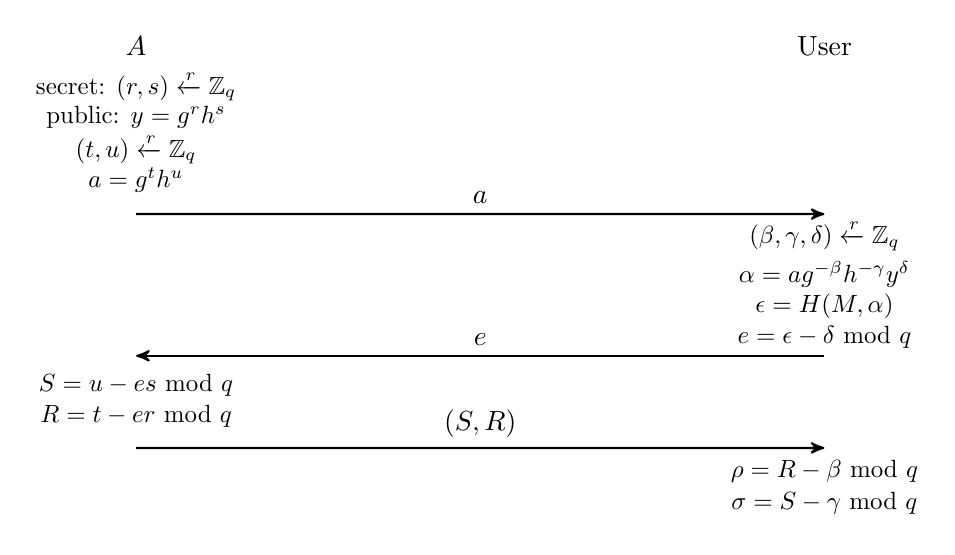
\begin{tikzpicture}[node distance=8cm,auto,>=stealth',scale=1,thick]
    \node[] (user) {User};
    \node[left = of user] (ca) {$A$};
    \node[below of=ca,scale=0.9, node distance=0.5cm] (ca_l1r1) {secret: $(r,s) \xleftarrow[]{r}\mathbb{Z}_q$};
    \node[below of=ca_l1r1,scale=0.9, node distance=0.4cm] (ca_l2r1) {public: $y=g^rh^s$};
    \node[below of=ca_l2r1,scale=0.9, node distance=0.4cm] (ca_l3r1) {$(t,u) \xleftarrow[]{r}\mathbb{Z}_q$};
    \node[below of=ca_l3r1,scale=0.9, node distance=0.4cm] (ca_l4r1) {$a = g^th^u$};
    \node[below of=ca_l4r1,scale=0.9, node distance=2cm] (ca_l1r3) {};
    \node[below of=ca_l1r3,scale=0.9, node distance=0.6cm] (ca_l2r3) {$S=u-es$ mod $q$};
    \node[below of=ca_l2r3,scale=0.9, node distance=0.4cm] (ca_l3r3) {$R=t-er$ mod $q$};
    \node[below of=ca_l3r3,scale=0.9, node distance=0.3cm] (ca_l4r3) {};
    \node[below of=ca,scale=0.9, node distance=6cm] (ca_ground) {};
    \node[below of=user,scale=0.9, node distance=1.7cm] (user_l1r2) {};
    \node[below of=user_l1r2,scale=0.9, node distance=0.7cm] (user_l2r2) {$(\beta, \gamma, \delta) \xleftarrow[]{r}\mathbb{Z}_q$};
    \node[below of=user_l2r2,scale=0.9, node distance=0.5cm] (user_l3r2) {$\alpha=ag^{-\beta} h^{-\gamma} y^\delta$};
    \node[below of=user_l3r2,scale=0.9, node distance=0.4cm] (user_l4r2) {$\epsilon=H(M,\alpha)$};
    \node[below of=user_l4r2,scale=0.9, node distance=0.4cm] (user_l5r2) {$e=\epsilon-\delta$ mod $q$};
    \node[below of=user_l5r2,scale=0.9, node distance=1.3cm] (user_l1r4) {};
    \node[below of=user_l1r4,scale=0.9, node distance=0.4cm] (user_l2r4) {$\rho=R-\beta$ mod $q$};
    \node[below of=user_l2r4,scale=0.9, node distance=0.4cm] (user_l3r4) {$\sigma=S-\gamma$ mod $q$};
    \node[below of=user,scale=0.9, node distance=6cm] (user_ground) {};
    %

    \draw[->] ($(ca_l4r1)!0.1!(ca_ground)$) -- node[above,scale=1,midway]{$a$} ($(user_l1r2)!0.1!(user_ground)$);
    \draw[<-] ($(ca_l1r3)!0.1!(ca_ground)$) -- node[above,scale=1,midway]{$e$} ($(user_l5r2)!0.1!(user_ground)$);
    \draw[->] ($(ca_l4r3)!0.1!(ca_ground)$) -- node[above,scale=1,midway]{$(S,R)$} ($(user_l1r4)!0.1!(user_ground)$);
\end{tikzpicture}}
\caption{Okamoto-Schnorr blind signature diagram, where $y \xleftarrow[]{r}\mathbb{Z}_q$ means that $y$ is randomly chosen in $\mathbb{Z}_q$.}
\label{dia:oss}
\end{figure*}

The Okamoto-Schnorr blind signature scheme is suitable with a private blockchain architecture due to the blinding process can be performed by the same authority responsible of the enrollment process (see Figure~\ref{dia:oss}, where the authority $A$ blindly signs a message for the user).

\subsection{Practical Byzantine Fault Tolerance (PBFT) Consensus Protocol}
\label{PBFT}
Practical Byzantine Fault Tolerance (PBFT) is a high-performance state machine replication protocol introduced by Miguel Castro and Barbara Liskov in 1999~\cite{castro1999practical}. This algorithm can be implemented for any replicated service within a distributed architecture, based on a local replica and some operations. These operations can be simple (i.e., read and write), or any other more sophisticated deterministic operations. The algorithm achieves liveness and safety with at most $\lfloor \frac{n-1}{3} \rfloor$ out of $n$ faulty replicas~\cite{castro1999practical}. This protocol is a practical implementation of a consensus algorithm capable of tolerating Byzantine Failure~\cite{lamport1982byzantine} on an asynchronous network. Although PBFT was implemented as a replication library for a file system, the design is practical enough to be considered as a faster and simpler alternative to others traditional consensus algorithm like Paxos~\cite{martin2006fast}. However, this consensus algorithm assumes common knowledge of the participant of the network, i.e., identities, as explained in~\cite{pass2017analysis}, making it unsuitable for some open decentralised systems, i.e., Permissionless Ledger.

\subsubsection{PBFT general description.}
The state machine replication algorithm purposed in PBFT is based on a consensus process between the nodes within a network arranged as a distributed system. The resiliency of the algorithm is optimal when the network has at least $3f+1$ replicas or nodes with up to $f$ of them faulty~\cite{bracha1985asynchronous}. The outnumber of replicas is necessary because we can reach consensus with the response of $n-f$ of them, where $f$ can be non-responding or faulty replicas, and $n$ the total number of replicas into the network. Moreover, it is possible that some of the responses considered in the consensus process coming from faulty replicas. Nevertheless, if the number of non-faulty replicas is outnumbering (i.e., $n-2f > f$), there are enough responses to consider that the protocol remains resilient against faulty replicas.

The algorithm is modelled so that each machine state replica has a local state and supports special operations to process the requests received from the network. The replicas or nodes are identified by enumerating them $\{0,...,\lvert R\rvert-1\}$, where $\lvert R\rvert=3f+1$ and $f$ is the maximum number of faulty replicas. The value of $R$ is selected to maintain the optimality of the algorithm because additional replicas can degrade the performance of the replication process. The replicas are organized in views, which correspond to a succession of configurations that are changing according to the liveness of the distributed system. The view configuration consists of one primary replica, and the rest of them are backups. The views are sorted by using consecutive numbers, and the primary replica $p$ is identified as $p=v\mod \lvert R\rvert$, where $v$ is the view number. The view changing holds if the primary begins to fail.

Before we start describing the protocol, we introduce the notation used in this paper. In any distributed system, the information is passing through the replicas or nodes within the network by using messages. Hence, we  denote a message by using $<\cdot,...,\cdot>$, where $\cdot$ corresponds to the message arguments. Moreover, we use the notation $(\cdot,...,\cdot)$ to group arguments inside a message.

The PBFT protocol consists of five steps. In other to keep the coherence with the original paper~\cite{castro1999practical}, we  use the same names of each step.

\begin{compactenum}
    \item \textbf{REQUEST:} In this stage, a client $c$ sends a \textit{REQUEST} message to the primary to execute an operation $o$ on the distributed system.
    \item \textbf{PRE-PREPARE:} After the primary receives the \textit{REQUEST} message, it validates the assign a sequence number $n$, then signs the message and finally sends it to the other backups in a \textit{PRE-PREPARE} message.
    \item \textbf{PREPARE:} The backups validate the operation $o$ indicated in the \textit{PRE-PREPARE} message, and then send its response in a signed message called \textit{PREPARE}.
    \item \textbf{COMMIT:} Replicas  send a \textit{COMMIT} message when they receive enough valid \textit{PREPARE} messages for the operation $o$.
    \item \textbf{REPLY:} Once the replicas have committed the operation $o$ they  send the result $r$ directly to the client $c$. Then the client $c$ accepts the result once it receives enough \textit{REPLY} messages with the same $r$ from different replicas.
\end{compactenum}

The process begins with a request sent by the client $c$ to execute an operation $o$ on the state machine. This process is carried out by sending a request message $m=<\textit{REQUEST},o,t,c,\sigma_c>$, where $t$ is a timestamp, and $\sigma_c$ is the signature of the message signed by the client $c$. Once the primary received the message $m$ starts the first phase of the algorithm called \textit{pre-prepare}. In this phase the primary assigns a reference number $n$ to the client request and creates a new message with structure $<(\textit{PRE-PREPARE},v,n,d,\sigma_p),m>$, where $v$ is the view number, $d$ is the digest of the message $m$, and $\sigma_p$ is the signature of the \textit{pre-prepare} message. Then the primary sends the pre-prepared message to the backups to continue the process. The backups accept the \textit{pre-prepare} message if:
\begin{itemize}
\item $\sigma_p$ and $\sigma_c$ are correct;
\item $d$ corresponds to the hash of the message $m$;
\item \textit{pre-prepare} message is in the view $v$;
\item The sequence number is within the range $[h,H]$ (to prevent that a faulty primary exhaust the sequence number selecting a large $n$);
\item the backup has not been accepted by another \textit{pre-prepare} message with sequence $n$ and view $v$ with a different $d$.
\end{itemize}

Once the backup $i$ has accepted the \textit{pre-prepare} message, it executes the \textit{prepare} phase broadcasting a message $<\textit{PREPARE},v,n,d,i,\sigma_i>$ to the other replicas (including the primary). 

A replica accepts the prepare message if:
\begin{itemize}
\item The signatures $\sigma_c$, $\sigma_p$ and $\sigma_i$ are correct;
\item The view number $v$ corresponds to the replica's view;
\item The sequence number $n$ is within $[h,H]$.
\end{itemize}

After the \textit{prepare} phase, a replica $k$ will enter to phase \textit{commit} after it has included in their log the request $m$, a \textit{pre-prepare} message for the request $m$ in the view $v$ with sequence number $n$, and $2f$ \textit{prepare} messages from different backups. In the \textit{commit} phase, the replica $k$  broadcasts a message $<\textit{COMMIT},v,n,d,k,\sigma_k>$ to the other replicas. The commit message is accepted by the replicas if:
\begin{itemize}
\item The signatures $\sigma_c$, $\sigma_p$, $\sigma_i$ and $\sigma_k$ are correct;
\item The view number $v$ corresponds to the replica's view;
\item The sequence number $n$ is within $[h,H]$.
\end{itemize}

The replica $l$ executes the operation $o$ requested by the client $c$ in the message $m$ once the \textit{prepare} phase has concluded in $f+1$ non-faulty replicas and has accepted $2f+1$ commit messages from other replicas with the same view $v$, sequence number $n$, and digest $d$. After the execution of the operation $o$, the replica $l$ generates a reply message $<\textit{REPLY},v,t,c,l,r,\sigma_l>$, where $r$ is the operation result, and then it is sent to the client.

Finally, the client accepts the result once it receives $f+1$ reply messages with valid signatures from different replicas with the same timestamp $t$ and result $r$.

\subsection{PBFT consensus in private blockchain implementations}
\label{PBFTHF}

The blockchain is a decentralised database organised in blocks that are appended one behind the other by using a hash pointer. Each block contains records that include the data to be stored into the chain. The blockchain design makes it suitable to be used as a distributed ledger, due to the record organisation inside a block (i.e., financial transactions) and the hash chain between blocks that makes it resistant to malicious modifications. As any other distributed system, blockchain needs a consensus algorithm to replicate the chain in each node member of the network. Nevertheless, the selections or design of the consensus algorithm must be aligned with the blockchain architecture and the openness of the system.

In this architecture, every user must be enrolled into the system through a Certificate Authority (CA) before joining the network. The Certificate Authority is responsible for generating the user credential for each new client and/or peer. This model provides a base of knowledge of the network members, making PBFT suitable for the blockchain replication process. Our consensus approach for permissioned ledger aims to the opposite of the permissionless replication protocol. The security of the consensus algorithm in a permissionless architecture is achieved proving the node honesty by expending their resources (i.e., computing capacity, power consumption, stakes, among others). In contrast, a PBFT-based protocol reaches the consensus accepting as valid the result proposed by the nodes majority.  A widely used PBFT-based consensus approach for blockchain is the native implementation made it for Hyperladger Fabric. 

This consensus algorithm is a novel version of PBFT based on an \textit{execute-order-validate} process~\cite{androulaki2018hyperledger}. In this protocol, each transaction passes through these three stages. The \textit{execution} phase triggers the transaction and then validates by endorsing it. In the \textit{order} phase, the transactions are ordered according to the consensus protocol. Finally, the \textbf{validation} phase checks the security policies per operation and application types.

The transactional flow on a permissioned blockchain can vary according to the consensus algorithm. In general, PBFT implementations are immersed in the whole transactional process and not only in the agreement of the new block. In the case of Hyperledger Fabric, a specific service leads the consensus~\cite{androulaki2018hyperledger}. However, the authentication and transaction validation are part of PBFT and are integrated into the whole transactional cycle.  

In the case of a blockchain PBFT-based consensus algorithms, we start with the clients $c_{bc}$ that has the same role than a client in the PBFT procotol. Then we have submitting peers $sp_{i_{bc}}$ that send the transaction proposal with the instructions sent by the client to the endorsing peers to validate the transaction. This process is similar than the executed by the primary in the PBFT algorithm, that sends the message with the instructions to the backups to validate it. Then, for the transaction endorsement, the endorsing peers send the response to the submitting peer to collect the responses after the validation process. Finally, the submitting peer sends the transaction to the orderers to propose a new block and then commit it for the network members. This process differs from the PBFT, where the backups respond to the other backups, all of them waits to have enough prepare and commit messages to then reply directly to the client, without pass through the primary. 

To exemplify this process, consider that we have a client $c_{bc}$ that needs to execute an operation $o_{bc}$ on a PBFT-based network. To process this request, we need to execute the following five steps: Initiating Transactions, Transaction Proposal, Transaction Endorsement, Broadcasting to Consensus and Commitment (see Figure~\ref{dia:pbft_BC}).

\begin{figure*}[tb]
\centering
\fbox{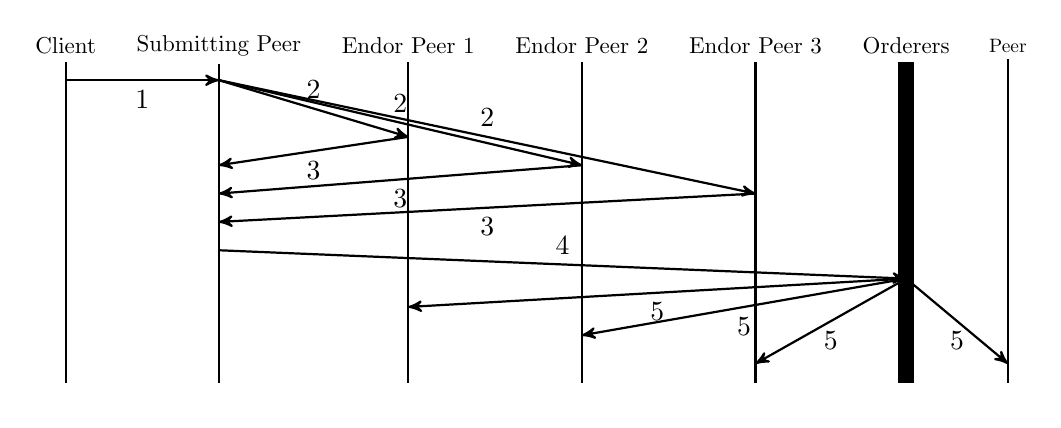
\begin{tikzpicture}[node distance=0.3cm,auto,>=stealth',scale=1,thick]
    %Nodes definition
    \node[scale=0.7] (peer) {Peer};
    \node[left = of peer, scale=0.83] (ord) {Orderers};
    \node[left = of ord, scale=0.83] (endp3) {Endor Peer 3};
    \node[left = of endp3,scale=0.83] (endp2) {Endor Peer 2};
    \node[left = of endp2,scale=0.83] (endp1) {Endor Peer 1};
    \node[left = of endp1, scale=0.83] (sp) {Submitting Peer};
    \node[left = of sp, scale=0.83] (client) {Client};
    \node[below of=client,scale=0.9, node distance=0.4cm] (client1) {};
    \node[below of=client1,scale=0.9, node distance=0.4cm] (client2) {};
    \node[below of=client2,scale=0.9, node distance=0.4cm] (client3) {};
    \node[below of=client3,scale=0.9, node distance=0.4cm] (client4) {};
    \node[below of=client4,scale=0.9, node distance=0.4cm] (client5) {};
    \node[below of=client5,scale=0.9, node distance=0.4cm] (client6) {};
    \node[below of=client6,scale=0.9, node distance=0.4cm] (client7) {};
    \node[below of=client7,scale=0.9, node distance=0.4cm] (client8) {};
    \node[below of=client8,scale=0.9, node distance=0.4cm] (client9) {};
    \node[below of=client9,scale=0.9, node distance=0.4cm] (client10) {};
    \node[below of=client10,scale=0.9, node distance=0.4cm] (client_ground) {};
    \node[below of=sp,scale=0.9, node distance=0.4cm] (sp1) {};
    \node[below of=sp1,scale=0.9, node distance=0.4cm] (sp2) {};
    \node[below of=sp2,scale=0.9, node distance=0.4cm] (sp3) {};
    \node[below of=sp3,scale=0.9, node distance=0.4cm] (sp4) {};
    \node[below of=sp4,scale=0.9, node distance=0.4cm] (sp5) {};
    \node[below of=sp5,scale=0.9, node distance=0.4cm] (sp6) {};
    \node[below of=sp6,scale=0.9, node distance=0.4cm] (sp7) {};
    \node[below of=sp7,scale=0.9, node distance=0.4cm] (sp8) {};
    \node[below of=sp8,scale=0.9, node distance=0.4cm] (sp9) {};
    \node[below of=sp9,scale=0.9, node distance=0.4cm] (sp10) {};
    \node[below of=sp10,scale=0.9, node distance=0.4cm] (sp_ground) {};
    \node[below of=endp1,scale=0.9, node distance=0.4cm] (endp11) {};
    \node[below of=endp11,scale=0.9, node distance=0.4cm] (endp12) {};
    \node[below of=endp12,scale=0.9, node distance=0.4cm] (endp13) {};
    \node[below of=endp13,scale=0.9, node distance=0.4cm] (endp14) {};
    \node[below of=endp14,scale=0.9, node distance=0.4cm] (endp15) {};
    \node[below of=endp15,scale=0.9, node distance=0.4cm] (endp16) {};
    \node[below of=endp16,scale=0.9, node distance=0.4cm] (endp17) {};
    \node[below of=endp17,scale=0.9, node distance=0.4cm] (endp18) {};
    \node[below of=endp18,scale=0.9, node distance=0.4cm] (endp19) {};
    \node[below of=endp19,scale=0.9, node distance=0.4cm] (endp110) {};
    \node[below of=endp110,scale=0.9, node distance=0.4cm] (endp1_ground) {};
    \node[below of=endp2,scale=0.9, node distance=0.4cm] (endp21) {};
    \node[below of=endp21,scale=0.9, node distance=0.4cm] (endp22) {};
    \node[below of=endp22,scale=0.9, node distance=0.4cm] (endp23) {};
    \node[below of=endp23,scale=0.9, node distance=0.4cm] (endp24) {};
    \node[below of=endp24,scale=0.9, node distance=0.4cm] (endp25) {};
    \node[below of=endp25,scale=0.9, node distance=0.4cm] (endp26) {};
    \node[below of=endp26,scale=0.9, node distance=0.4cm] (endp27) {};
    \node[below of=endp27,scale=0.9, node distance=0.4cm] (endp28) {};
    \node[below of=endp28,scale=0.9, node distance=0.4cm] (endp29) {};
    \node[below of=endp29,scale=0.9, node distance=0.4cm] (endp210) {};
    \node[below of=endp210,scale=0.9, node distance=0.4cm] (endp2_ground) {};
    \node[below of=endp3,scale=0.9, node distance=0.4cm] (endp31) {};
    \node[below of=endp31,scale=0.9, node distance=0.4cm] (endp32) {};
    \node[below of=endp32,scale=0.9, node distance=0.4cm] (endp33) {};
    \node[below of=endp33,scale=0.9, node distance=0.4cm] (endp34) {};
    \node[below of=endp34,scale=0.9, node distance=0.4cm] (endp35) {};
    \node[below of=endp35,scale=0.9, node distance=0.4cm] (endp36) {};
    \node[below of=endp36,scale=0.9, node distance=0.4cm] (endp37) {};
    \node[below of=endp37,scale=0.9, node distance=0.4cm] (endp38) {};
    \node[below of=endp38,scale=0.9, node distance=0.4cm] (endp39) {};
    \node[below of=endp39,scale=0.9, node distance=0.4cm] (endp310) {};
    \node[below of=endp310,scale=0.9, node distance=0.4cm] (endp3_ground) {};
    \node[below of=ord,scale=0.9, node distance=0.4cm] (ord1) {};
    \node[below of=ord1,scale=0.9, node distance=0.4cm] (ord2) {};
    \node[below of=ord2,scale=0.9, node distance=0.4cm] (ord3) {};
    \node[below of=ord3,scale=0.9, node distance=0.4cm] (ord4) {};
    \node[below of=ord4,scale=0.9, node distance=0.4cm] (ord5) {};
    \node[below of=ord5,scale=0.9, node distance=0.4cm] (ord6) {};
    \node[below of=ord6,scale=0.9, node distance=0.4cm] (ord7) {};
    \node[below of=ord7,scale=0.9, node distance=0.4cm] (ord8) {};
    \node[below of=ord8,scale=0.9, node distance=0.4cm] (ord9) {};
    \node[below of=ord9,scale=0.9, node distance=0.4cm] (ord10) {};
    \node[below of=ord10,scale=0.9, node distance=0.4cm] (ord_ground) {};
    \node[below of=peer,scale=0.9, node distance=0.4cm] (peer1) {};
    \node[below of=peer1,scale=0.9, node distance=0.4cm] (peer2) {};
    \node[below of=peer2,scale=0.9, node distance=0.4cm] (peer3) {};
    \node[below of=peer3,scale=0.9, node distance=0.4cm] (peer4) {};
    \node[below of=peer4,scale=0.9, node distance=0.4cm] (peer5) {};
    \node[below of=peer5,scale=0.9, node distance=0.4cm] (peer6) {};
    \node[below of=peer6,scale=0.9, node distance=0.4cm] (peer7) {};
    \node[below of=peer7,scale=0.9, node distance=0.4cm] (peer8) {};
    \node[below of=peer8,scale=0.9, node distance=0.4cm] (peer9) {};
    \node[below of=peer9,scale=0.9, node distance=0.4cm] (peer10) {};
    \node[below of=peer10,scale=0.9, node distance=0.4cm] (peer_ground) {};

    % Vertical Lines
    \draw (client) -- (client_ground);
    \draw (sp) -- (sp_ground);
    \draw (endp1) -- (endp1_ground);
    \draw (endp2) -- (endp2_ground);
    \draw (endp3) -- (endp3_ground);
    \draw[line width=0.2cm] (ord) -- (ord_ground);
    \draw (peer) -- (peer_ground);

    %Initiating Transactions
    \draw[->] ($(client)!0.1!(client_ground)$) -- node[below,scale=1,midway]{$1$} ($(sp)!0.1!(sp_ground)$);
    %Transaction Proposal
    \draw[->] ($(sp)!0.1!(sp_ground)$) -- node[above,scale=1,midway]{$2$} ($(endp12)!0.1!(endp1_ground)$);
    \draw[->] ($(sp)!0.1!(sp_ground)$) -- node[above,scale=1,midway]{$2$} ($(endp23)!0.1!(endp2_ground)$);
    \draw[->] ($(sp)!0.1!(sp_ground)$) -- node[above,scale=1,midway]{$2$} ($(endp34)!0.1!(endp3_ground)$);

    %Endorsing Transactions
    \draw[->] ($(endp12)!0.1!(endp1_ground)$) -- node[below,scale=1,midway]{$3$} ($(sp3)!0.1!(sp_ground)$);
    \draw[->] ($(endp23)!0.1!(endp2_ground)$) -- node[below,scale=1,midway]{$3$} ($(sp4)!0.1!(sp_ground)$);
    \draw[->] ($(endp34)!0.1!(endp3_ground)$) -- node[below,scale=1,midway]{$3$} ($(sp5)!0.1!(sp_ground)$);
    %Broadcasting to Consensus
    \draw[->] ($(sp6)!0.1!(sp_ground)$) -- node[above,scale=1,midway]{$4$} ($(ord7)!0.1!(ord_ground)$);
    %Commit
    \draw[->] ($(ord7)!0.1!(ord_ground)$) -- node[below,scale=1,midway]{$5$} ($(endp18)!0.1!(endp1_ground)$);
    \draw[->] ($(ord7)!0.1!(ord_ground)$) -- node[below,scale=1,midway]{$5$} ($(endp29)!0.1!(endp2_ground)$);
    \draw[->] ($(ord7)!0.1!(ord_ground)$) -- node[below,scale=1,midway]{$5$} ($(endp310)!0.1!(endp3_ground)$);
    \draw[->] ($(ord7)!0.1!(ord_ground)$) -- node[below,scale=1,midway]{$5$} ($(peer10)!0.1!(peer_ground)$);
    
\end{tikzpicture}}
\caption{Transaction Flow~\cite{androulaki2018hyperledger}.}
\label{dia:pbft_BC}
\end{figure*}


\Par{\textit{\textbf{Initiating Transactions:}}}
In the initiating transactions, the client $c_{bc}$ generates a message to invoke specific operation $o_{bc}$ to be resolved by the network. The message is sent to a submitting peer, then we continue with the process. In the case that the submitting peer is offline or misbehaviour, the client sends the transaction to the next submitting peer. The structure of the message is presented below:~\\

\noindent\fbox{\begin{minipage}[c]{0.475\textwidth}
$<\textit{SUBMIT},c_{bc},o_{bc},txPayload,\sigma_c,retryFlag>$, where:
\begin{itemize}
\item $c_{bc}$: is the client ID,
\item $o_{bc}$: refers to the operation inside the distributed system,
\item $txPayload$: is the payload of the submitted transaction,
\item $\sigma_c$: is signature of a client,
\item $retryFlag$: boolean variable to identify whether to retry the submission of the transaction in case of the transaction fails. 
\end{itemize}
\end{minipage}}

\Par{\textit{\textbf{Transaction Proposal:}}}
The submitter peer ($sp_{bc}$) receives the transaction and verifies the client signature $\sigma_{c}$. Then prepares a transaction proposal to be sent to the endorsing peer. The transaction proposal consists of invoking the operations $o_{bc}$ and compute the state update (\textit{stateUpdate}) and version dependency ($\textit{verDep}$). The version dependencies relate the variables involve in the transaction with his version in the state and their respective operation. For example: if a client wants to read and write in the blockchain, the version dependency is a tuple $\left(readset,writeset\right)$ where:

\begin{itemize}
\item for every variable $k$ read by the transaction, the pair $(k,s(k).version)$ is added to readset,
\item for every variable $k$ modified by the transaction, the pair $(k,s(k).version)$ is added to $writeset$.
\end{itemize}

Once the execution of the proposal is done, the submitter peer generates the \textit{transaction proposal} message, defined as: ~\\

\noindent\fbox{\begin{minipage}[c]{0.475\textwidth}
$<\textit{PROPOSAL},m_c,trans_{prop}>$, where:
\begin{itemize}
\item $m_c$:= $\left(c_{bc},o_{bc},txPayload,\sigma_c\right)$,
\item $trans_{prop}$:= $(sp_{bc},o_{bc},txContentBlob,stateUpdate,$ $verDep)$
\end{itemize}
\end{minipage}}

\Par{\textit{\textbf{Transaction Endorsement:}}} The endorser peer ($ep_{bc}$) verifies the client signature $\sigma_c$ coming in $m_c$ and checks that the operation $o_{bn}$ in $m_c$ and $trans_{prop}$ is the same. Then, the endorser simulates the transaction proposal and validates that the $stateUpdate$ and $verDep$ are correct. If the validation process is successful, the endorser peer generates a \textit{transaction valid} message to be sent to the submitter peer. The message has the following structure: ~\\

\noindent\fbox{\begin{minipage}[c]{0.475\textwidth}
$<\textit{TRANSACTION-VALID},tx_{id},\sigma_{ep}>$, where:
\begin{itemize}
\item $tx_{id}$: is the transaction identifier generated with the client ID and a nonce,
\item $\sigma_ep$:= is signature of the message signed by the submitter peer $sp_{BC}$.
\end{itemize}
\end{minipage}}

In the case of the simulation process ends unsuccessfully, the endorser peer generates a \textit{transaction invalid} message: ~\\

\noindent\fbox{\begin{minipage}[c]{0.475\textwidth}
$<\textit{TRANSACTION-INVALID},tx_{id},Error,\sigma_{ep}>$, where \textit{Error} can be:
\begin{itemize}
\item \textit{INCORRECT-STATE}: when the endorser obtains a different \textit{state update} than the one coming in the \textit{transaction proposal},
\item \textit{INCORRECT-VERSION}: when there is the newest version of the variable referred in the \textit{transaction proposal},
\item \textit{REJECTED}: for any other reason.
\end{itemize}
\end{minipage}}

\Par{\textit{\textbf{Broadcasting to Consensus:}}} The submitter peer waits for the response from the endorsing peers. When it receives enough \textit{Transaction Valid} messages adequately signed, the peer stores the endorsing signatures into packaged called \textit{endorsement}. Once the transaction is considered endorsed, the peer invokes the consensus services by using \textit{broadcast(blob)}, where \textit{blob:=(trans\textsubscript{prop}}, \textit{endorsement)}.

The number of responses and endorsing to consider the \textit{transaction proposal} as endorsed depends on the configuration of the permissioned blockchain. If the transaction has failed to collect the enough endorsements, it abandons this transaction and notifies to the submitter.

\Par{\textit{\textbf{Commitment:}}} Once a submitter peer broadcast transactions properly endorsed to consensus, an ordering services collects these transactions into blocks. From the ordering service, we get a hash-chained sequence of blocks with the transactions endorsed. The block prepared by the ordering service has the form $B=\left(\left[tx_1,tx_2,...,tx_k\right],h\right)$, where $h$ corresponds to hash value of the previous block.

The peers receive the blocks from the ordering service through a direct connection or by using a gossip protocol. Once the peers have the new block, they  check if the endorsement of each transaction is valid according to the policy configured in the network. Then, it verifies the \textit{verDep} in order to ensure there are no conflicts between the operation $o_{bc}$; the variables involved in the transaction and the current \textit{state}. If this process finishes successfully, the transactions are committed. In the case that one of the validation fails, the peer considers the transaction as invalid and drops it. Finally, the invalid transactions are informed to the client $c_{bc}$ by the submitter peer $sp_{bc}$, and according to the \textit{retryFlag}, the $sp_{bc}$ may retry the transaction.

The peers can change the local state just once the transactions are committed. Hence, the peer into the network will update their local version of the ledger once all the transactions in the block are committed. Finally, the state update is done by appending the new block to their local version of the blockchain.

\section{Privacy Preserving PBFT for Permissioned Ledgers}\label{PPPBFT}

Considering a permissioned PBFT based consensus protocol like the one introduced in Section~\ref{PBFTHF}, in this protocol, we use the digital signature as user authentication method without protecting the user privacy. Hence, for a privacy preserving consensus protocol, we need to have the following properties:

\begin{itemize}
    \item Alice sends a newly signed transaction to the CA,
    \item Alice’ signature is validated only by the CA,
    \item The CA signs the transaction proposed by Alice and anonymizes Alice’s identity,
    \item The CA signs the transaction sent by Alice to the network,
    \item all the nodes members of the transactions validation process can validate the CA's signature,
    \item the CA signature cannot be duplicated.
\end{itemize}

Now, to keep the privacy of the client and peers involved in the transactional process, we need to hide his ID and blind his signature. However, we do not address the ID hiding process with any particular mechanism. Therefore, we consider that the ID is replaced by a value corresponding to the anonymized user ID, and this process can be performed by using different schemes.

To address the issue related to the digital signature, we will replace the signing mechanism used in the original protocol by the Okamoto-Schnorr blind signature scheme~\cite{okamoto1992provably}. By recapitulating the consensus protocol above mentioned, the transactional process consists of the follows steps:

\begin{enumerate}
    \item \textbf{Initiating Transactions:} The client $c_{bc}$ generates a signed message to execute an operation $o_{bc}$ in the network.
    \item \textbf{Transaction Proposal:} The submitting peer $sp_{bc}$ receives the message coming from the client $c_{bc}$, validates the client signature and propose a blockchain transaction with the client instruction $o_{bc}$.
    \item \textbf{Transaction Endorsement:} The endorser peer $ep_{bc}$ validates the client $c_{bc}$ signatures and verifies that the transaction is correctly simulating the operation $o_{bc}$ using his local version of the blockchain. Then, he generates the signed transactions with the result of the validation process and sends it to the submitting peer $sp_{bc}$.
    \item \textbf{Broadcasting to Consensus:} The submitting peer $sp_{bc}$ collects the endorse coming from the endorser peers connected to the network. Once $sp_{bc}$ collects enough valid answers from the endorsers, he broadcasts the transaction proposal with the endorsement to the ordering service.
    \item \textbf{Commitment:} All the transactions are ordered within a block, and are validated with their respective endorsement. Then, the new block is spread through the network to be committed by the peers.
\end{enumerate}

In order to maintain the consistency and liveness that the protocol has, we keep the transactional flow. However, the steps are modified in order to accept the new blind signature scheme to authenticate the clients and peers.

We define three new functions to represent the signing process and the operation execution inside the protocol. Let $BlindSign(M,(\beta,\sigma,\gamma),y)$ and \textit{VerifyBlindSign(M,}$(\rho,\delta,\epsilon),y)$ be the functions to sign blind and to verify the blind signature, respectively. Where $M$ corresponds to the message to be signed, $(\beta,\sigma,\gamma)$ to the secret values randomly chosen $(\xleftarrow[]{r}\mathbb{Z}_q)$ by the client or peer, $(\rho,\delta,\epsilon)$ to the blind signature; and $y$ to the CA public key. The result obtained from the function \textit{BlindSign} corresponds to the blind signature $(\rho,\sigma,\epsilon)$. On the other hand, the function \textit{VerifyBlindSign} returns a response \textit{valid} or \textit{invalid}. The third function corresponds to \textit{EXEC(o,Payload)}, and represents the execution process of the operation $o$ on \textit{Payload} performed by the peer. Additionally, we use the variables \textit{tid} as the transaction ID, \textit{SecurityPolicies} to define the set of security parameters configured in the node for the operation $o_{bc}$ (i.e., read and write rights), and \textit{TotEndorPeers} for the total number of endorsing peers in the network.

Now that we already have defined the functions and the variables used in the protocol, we need to integrate it inside of each step of the transactional flow. The transactional process starts with the function \textbf{Initiating Transactions} described in Algorithm~\ref{alg:InitTx}. In this step, we replace the client ID by a random number, then we concatenate the arguments $(crand,o_{bc},Payload,retryFlag)$ to be signed, and then we use the function \textit{BlindSign} to generate the blind signature according to the protocol described in Section~\ref{Okamoto}. Finally, we generate the message \textit{SUBMIT} to be sent to the submitting peer $sp_{bc}$.

\begin{algorithm}[ht]
\caption{InitTx($o_{bc}$,$Payload$,$retryFlag$,$y$)}
\label{alg:InitTx}
\begin{algorithmic}[1]
\STATE $crand_{bc}\xleftarrow[]{r}\mathbb{N}$            
\STATE $M \gets (crand||o_{bc}||Payload,retryFlag)$
\STATE $(\beta,\gamma,\delta)\xleftarrow[]{r}\mathbb{Z}_q$  
\STATE $(\rho,\sigma,\epsilon) \gets BlindSign(M,(\beta,\gamma,\delta),y)$
\RETURN $<\textit{SUBMIT},crand_{bc},o_{bc},Payload,retryFlag,$ $(\rho,\sigma,\epsilon)>$
\end{algorithmic}
\end{algorithm}

The second step corresponds to the \textbf{Transaction Proposal} (see Algorithm~\ref{alg:TxProp}). In this process we start by validating the blind signature by using the function $VerifyBlidnSign(M,(\rho,\sigma,\epsilon),y)$, where $M$ is the signed message, $(\rho,\sigma,\epsilon)$ is the blind signature, and $y$ is the CA public key. In the case that the validation process fails, the function rejects the transaction; otherwise, the peer executes the operation $o_{bc}$ on the \textit{Payload}, and finally gets $verDep$ and $stateUpdate$. Finally, the submitting peer generates the \textit{PROPOSE} message to be sent to the endorsers.

\begin{algorithm}[ht]
\caption{TxProp($crand_{bc},sp_{bc},o_{bc},Payload,retryFlag,$ $(\rho,\sigma,\epsilon),y$)}
\label{alg:TxProp}
\begin{algorithmic}[1]
\STATE $m \gets (crand_{bc},o_{bc},Payload,retryFlag,(\rho,\sigma,\epsilon))$
\STATE $M \gets (crand,o_{bc}||Payload||retryFlag)$
\IF{$VerifyBlindSign(M,(\rho,\sigma,\epsilon),y) == invalid$}  \RETURN $invalid$ \ELSE
\STATE $(verDep,stateUpdate) \gets EXEC(o_{{bc}},Payload)$ 
\STATE $trans_{prop} \gets (sp_{bc},o_{bc},Payload,stateUpdate,$ $verDep)$
\RETURN $<\textit{PROPOSE},m,trans_{prop}>$
\ENDIF
\end{algorithmic}
\end{algorithm}

The next step corresponds to the \textbf{Transaction Endorsement} detailed in Algorithm~\ref{alg:TxEndors}. We start this process validating the blind signature using the function \textit{VerifyBlindSign} for the message $M=(.crand\vert\vert o_{bc} \vert\vert Payload \vert\vert retryFlag)$, the signature $(\rho,\sigma,\epsilon)$, and the CA public key $y$. In the case that the response is valid, we continue validating the \textit{verDep}, \textit{stateUpdate}, and the \textit{securityPolicies}. In the case that the \textit{verDep} corresponds to the last version that the endorsing peer has locally, and the \textit{stateUpdate} is the same that it has as local state, and the \textit{securityPolicies} authorizes the instruction $o$, we endorse the transaction; otherwise, we reject. To endorse the transaction, we use the function \textit{BlindSign} to sign the message \textit{TRANSACTION-VALID} with his corresponding $tid$. Finally, once the transaction is endorsed, the endorser peer creates the \textit{TRANSACTION-VALID} message to be sent to the submitting peer $sp_{bc}$.

\begin{algorithm}[ht]
\caption{TxEndors($m,trans_{prop},securityPolicies,y$)}
\label{alg:TxEndors}
\begin{algorithmic}[1]
\STATE $tid \gets m.Payload.tid$
\STATE $M \gets (m.crand\vert\vert m.o_{bc} \vert\vert m.Payload \vert\vert m.retryFlag)$
\IF{$VerifyBlindSign(M,(m.\rho,m.\sigma,m.\epsilon),y)$ \emph{== invalid}}  \RETURN \emph{invalid} \ELSE
\STATE ($verDep_{endorser}$,$stateUpdate_{endorser}$) $\gets$  \emph{EXEC(}$m.o_{bc}$\emph{,Payload)} \ENDIF
\STATE $(\beta,\gamma,\delta)\xleftarrow[]{r}\mathbb{Z}_q$  
\IF{$trans_{prop}.stateUpdate \neq stateUpdate_{endorser}$} 
\STATE \emph{result} $\gets$ \emph{(\textit{TRANSACTION-INVALID}||tid||\textit{INCORRECT-STATE})}
\STATE $(\rho,\sigma,\epsilon)_{ep} \gets BlindSign(result,(\beta,\gamma,\delta),y)$
\RETURN \emph{<\textit{TRANSACTION-INVALID},tid,\textit{INCORRECT-STATE},} $\sigma_{ep}>$ 
\ELSIF {$trans_{prop}.varDep \neq varDep_{endorser}$} 
\STATE \emph{result} $\gets$ \emph{(\textit{TRANSACTION-INVALID}||tid||\textit{INCORRECT-VERSION})}
\STATE $(\rho,\sigma,\epsilon)_{ep} \gets BlindSign(result,(\beta,\gamma,\delta),y)$
\RETURN \emph{<\textit{TRANSACTION-INVALID},tid,\textit{INCORRECT-VERSION},} $\sigma_{ep}>$ 
\ELSIF {$securityPolicies = invalid$} 
\STATE \emph{result} $\gets$ \emph{(\textit{TRANSACTION-INVALID}||tid||\textit{REJECTED})}
\STATE $(\rho,\sigma,\epsilon)_{ep} \gets BlindSign(result,(\beta,\gamma,\delta),y)$
\RETURN \emph{<\textit{TRANSACTION-INVALID},tid,\textit{REJECTED},} $\sigma_{ep}>$
\ELSE  
\STATE $result \gets (\textit{TRANSACTION-VALID}||tid)$
\STATE $(\rho,\sigma,\epsilon)_{ep} \gets BlindSign(result,(\beta,\gamma,\delta),y)$
\RETURN $<\textit{TRANSACTION-VALID},tid,\sigma_{ep}>$
\ENDIF
\end{algorithmic}
\end{algorithm}

Then, the submitting peer $sp_{bc}$ receives the responses from the endorsing peers during the \textbf{Broadcasting to Consensus} step (see Algorithm~\ref{alg:TxBrodCons}). These responses are collected inside of an array called \textit{endorsement}. Once the submitting peer has collected enough valid responses in the \textit{endorsement} array (at least $50\%+1$), it sends the transaction to the orderers to be included into the next block by using the function \textit{broadcast}. 

\begin{algorithm}[ht]
\caption{TxBrodCons($trans_{prop}$, $(\rho,\sigma,\epsilon_{ep})$, $endorsement_{tid}$)}
\label{alg:TxBrodCons}
\begin{algorithmic}[1]
\STATE $endorsment_{tid}[endorsement_{tid}.length+1]$ $\gets$ $(\rho,\sigma,\epsilon)_{ep}$
\IF{($endorsment_{tid}.length >= (\frac{TotEndorPeers}{2}+1$))}
\STATE $blob \gets (trans_{prop},endorsment_{tid})$
\RETURN $broadcast(blob)$
\ENDIF
\end{algorithmic}
\end{algorithm}

Finally, during the \textbf{Commitment} (see Algorithm~\ref{alg:BlockCommitment}) the transaction is validated with his respective endorsement. If the $verDep$ has not changed during the validation process and the $endorsement$ is valid according to the security policies for the operation $o_{bc}$, the transaction is added into the new block. The \textit{NewBlock} is an array where we store the new transactions to be settled, and once we reach the maximum block size (\textit{BlockLengthMax}) configured in the network, we spread the block to be committed by the peers using the function \textit{Commit2Network}. In the case that the validation process fails, the transition is rejected and the \textit{retryFlag} is set to 1. 

\begin{algorithm}[ht]
\caption{BlockCommitment(\emph{blob, NewBlock, securityPolicies, retryFlag)}}
\label{alg:BlockCommitment}
\begin{algorithmic}[1]
\IF{$(blob.endorsment_{tid} \notin securityPolicies)$ || $(blob.trans_{prop}.verDep \neq valid)$}
\RETURN $retryFlag \gets 1$
\ELSE \STATE $NewBlock [NewBlock.length + 1] \gets trans_{prop}$ \ENDIF
\IF{$NewBlock.lenght == BlockLengthMax$}
\RETURN $Commit2Network(B)$ \ENDIF
\end{algorithmic}
\end{algorithm}

\section{Protocol Properties}
\label{PROP}

\name{} has the following security properties.

\subsection{Consistency}
A protocol is said to be \emph{consistent} if the protocol has  to ensure that a transaction generated by a valid user stays settled adequately in the blockchain.

\begin{definition}
A protocol $\mathbb{P}$ is $T-consistent$ if a transaction $tx$ generated by an honest client $c_{cb}$ to execute a valid operation $o_{bc}$, it is confirmed into the network after $T-round$ of new blocks.
\end{definition}

\begin{theorem} \name{} protocol is 1-consistent.
\end{theorem}

\begin{proof}
The protocol described in Section \ref{PPPBFT} is a BFT based consensus algorithm. Consistency is achieved by agreeing with the validity of the transaction through a Byzantine Agreement process. Hence, for a transaction $tx$ that has reach a majority of valid endorses for a operation $o_{bc}$, the probability to not settle it in a new block and to have forks in the chain is neglected if we have at most $\lfloor\frac{n-1}{3}\rfloor$ out of total $n$ malicious peers, as it has been shown in~\cite{castro1999practical,li2007beyond} under the terminology of safeness. It is 1-consistent because we do not have any fork so only  one block is needed to wait in order to have a transaction validated.
\end{proof}

\subsection{Liveness}

The liveness property means that a consensus protocol ensures that if an honest client  submitting a peer is broadcasting a valid transaction, a new block is appended to the chain with the transaction. Hence, the protocol must ensure that the blockchain  growths if the valid clients generate valid transactions.

\begin{definition}[Liveness]
A consensus protocol $\mathbb{P}$ ensures \emph{liveness for a blockchain $C$} if $\mathbb{P}$ ensures that after a period of time $t$, the new version of the blockchain $C'$ is $C' > C$, if a valid client $c_{i_{bc}}$ has broadcasted a valid transaction $tx_i$ during the time $t$. 
\end{definition}

\begin{theorem}
\name{} achieves liveness.
\end{theorem}

\begin{IEEEproof}
\name{} is a PBTF-based consensus protocol. Thus, liveness is achieved if after the transaction validation process, the ordering services propose a new block $B$ with the transactions broadcasted by a client during a period of time $t$. Hence, for valid transactions $tx_i$, where $i\in \mathbb{N}_0$, issued by valid a client $c_{i_{bc}}$ during a period of time $t$, the probability that $C'= C$ is neglected if we have at most $\lfloor\frac{n-1}{3}\rfloor$ out of total $n$ malicious peers~\cite{castro1999practical}.
\end{IEEEproof}

\subsection{Blindness}

We use the definition of \emph{blindess} defined by Chaum and Pedersen in~\cite{10.1007/3-540-48071-4_7}, and Schnorr in~\cite{schnorr2001security}. A signature is properly blinded if the signer cannot get any information about the signature if the receiver follows the protocol correctly.

\begin{definition}[Blind signature]
A signing scheme is \emph{blind} if the signature $(m,\rho,\sigma,\epsilon)$ generated by following the protocol, correctly, is statistically independent of the interaction $(a,e,R,S)$ with that provides the view to the signer.
\end{definition}

\begin{theorem}
Okamoto-Schnorr signature $(m,\rho,\delta,\epsilon)$ is statistically independent to the interaction $(a,e,R,S)$ between the authority $A$ and the user.
\end{theorem}

\begin{IEEEproof}
We recall how the protocol works. To generate a blind signature $(m,\rho,\sigma,\epsilon)$ the user chooses randomly $(\beta,\gamma,\delta)\in \mathbb{Z}_q$ to response to the CA's commitment $a$ with the challenge $c=H(m,ag^\beta h^\gamma y^\delta) -\delta$ mod $q$. Then the CA sends $(R,S)=(t-er,u-es)$ to finally obtain the signature by calculating $(\rho,\sigma)=(R-\beta,S-\gamma)$.
Hence, for the constant interaction $(a,e,R,S)$ and a unique set $(\beta,\gamma,\delta)$ is randomly chosen per signature, we generate a signature $(m,\rho,\delta,\epsilon)=(m,R-\beta,S-\gamma,e+\gamma)$ that is uniformly distributed over all the signature of $m$ due to the random $(\beta,\gamma,\delta) \gets \mathbb{Z}_q$ \cite{schnorr2001security}.
\end{IEEEproof}

\subsection{Non-forgeability}
The non-forgeability property used in this paper refers to the impossibility for a user to compute a $k+1$ signature on his own after $k$ interactions with a signer; this proves that the only method to generate a valid signature is contacting the CA. This property was proved by Pointcheval and Stern in \cite{pointcheval1996provably}.

\begin{definition}[One more forgery]
For any integer \textit{k}, a PPT Turing machine \textit{A} can calculates $k+1$ signatures after \textit{k} interactions with the signer $\Sigma$ with non-negligible probability.  
\end{definition}

\begin{theorem}
Let Okamoto-Schnorr blind signature be a cryptographic scheme in the random oracle model. If there is a PPT Turing machine able to calculate a "one more" forgery with non-negligible probability (even with parallel attack), then the discrete logarithm can be solved in polynomial time.
\end{theorem}

\begin{IEEEproof}
Outline of the proof is detailed in~\cite{pointcheval1996provably}.
Consider that the public values $p$, $q$, $g$ and $h$; the secret keys $(r,s)$ and the public key $y$ are the same as described in Section~\ref{Okamoto}. Let \textit{Q} be a polynomial number that represents the queries asked to the random oracle ($\mathcal{Q}_1,...,\mathcal{Q}_Q$).

Let \textit{A} be the attacker. \textit{A} is a PPT Turing machine which success in computing  $l+1$ valid forgeries $(m_i,\alpha_i,\rho_i,\sigma_i,\epsilon_i)$ after $(a_i,e_i,R_i,S_i)$ interactions (see Section~\ref{Okamoto}) for $i\in\{i,...,k\}$ with non-negligible probability $\epsilon$.

We want to calculate the  discrete logarithm of $h$ relatively to $g$ by using oracle reply~\cite{10.1007/3-540-68339-9_33}, with the CA and the attacker colluded. We start running the attack with random keys, random tape $\Omega$ and oracle \textit{f}. Then we choose a random index \textit{j}', and we replay the attack using the same keys and tape but with different oracle ($f'$) such that the first $j-1$ answers do not change. We expect to obtain from both processes a common $\alpha_i$ from the $j^{th}$ query with different representations regarding $g$ and $h$, with non-negligible probability. Finally, the probability of success is bigger than (for more details see~\cite{pointcheval1996provably}):
\begin{equation}
    \frac{1}{2(k+1)}\left(\frac{1}{6(k+1)}\frac{\epsilon}{Q^{k+1}}\right)^3
\end{equation}
\end{IEEEproof}

\section{Conclusion} \label{conclu}
In this paper, we propose a new consensus algorithm for user identity privacy preserving. This algorithm is based on PBFT and Hyperledger Fabric algorithms. Our algorithm allows the users to issue a blind signature that keeps their identity private during the blockchain transaction validation process and after the transaction is settled. The signing scheme is based on Okamoto-Schnorr blind signature that is a provably secure \cite{pointcheval1996provably} and efficient signing scheme \cite{schnorr1991efficient}. The protocol was designed to implement a blind signature scheme by using the components that any permissioned or private blockchain architecture has. Hence, our algorithm performs the signature blinding process by using the CA that already exists in the permissioned scheme, making it efficient to be implemented in these kinds of blockchain architectures.

One open issue is the network privacy. Our protocol is vulnerable to user tracking through the network. Hence, the network privacy is an issue that is not addressed by \name{}. However, as a future work, we would like to integrate Mixnets~\cite{Chaum:1981:UEM:358549.358563} as decentralised application to hide the transaction source and accomplish privacy at a network level.

\bibliographystyle{plain}
\bibliography{nicfg.bib}

\end{document}